\documentclass{article}
\usepackage{graphicx} % Required for inserting images
\usepackage{multicol}
\graphicspath{{images/}} % configuring the graphicx package
\title{ACTORS DETECTION AND RETRIEVAL IN MOVIE SCENES}
\author{Bianco Michael, Bertolini Matteo, Todaro Marco}
\date{April 2023}

\begin{document}
\maketitle
\section{Introduction}

Our idea is to build a deep learning algorithm to recognize and detect celebrities acting in different 
movie scenes, 
even if they are dressed up, made up or in movement.
The literature necessary to work on this kind of model requires the study of convolutional neural networks
for extracting the most salient features useful to describe each actor we are recognizing and algorithms for edge
detection, in particular for face detection.

\begin{center}
\begin{multicols}{2}
\vspace*{-0.4in}
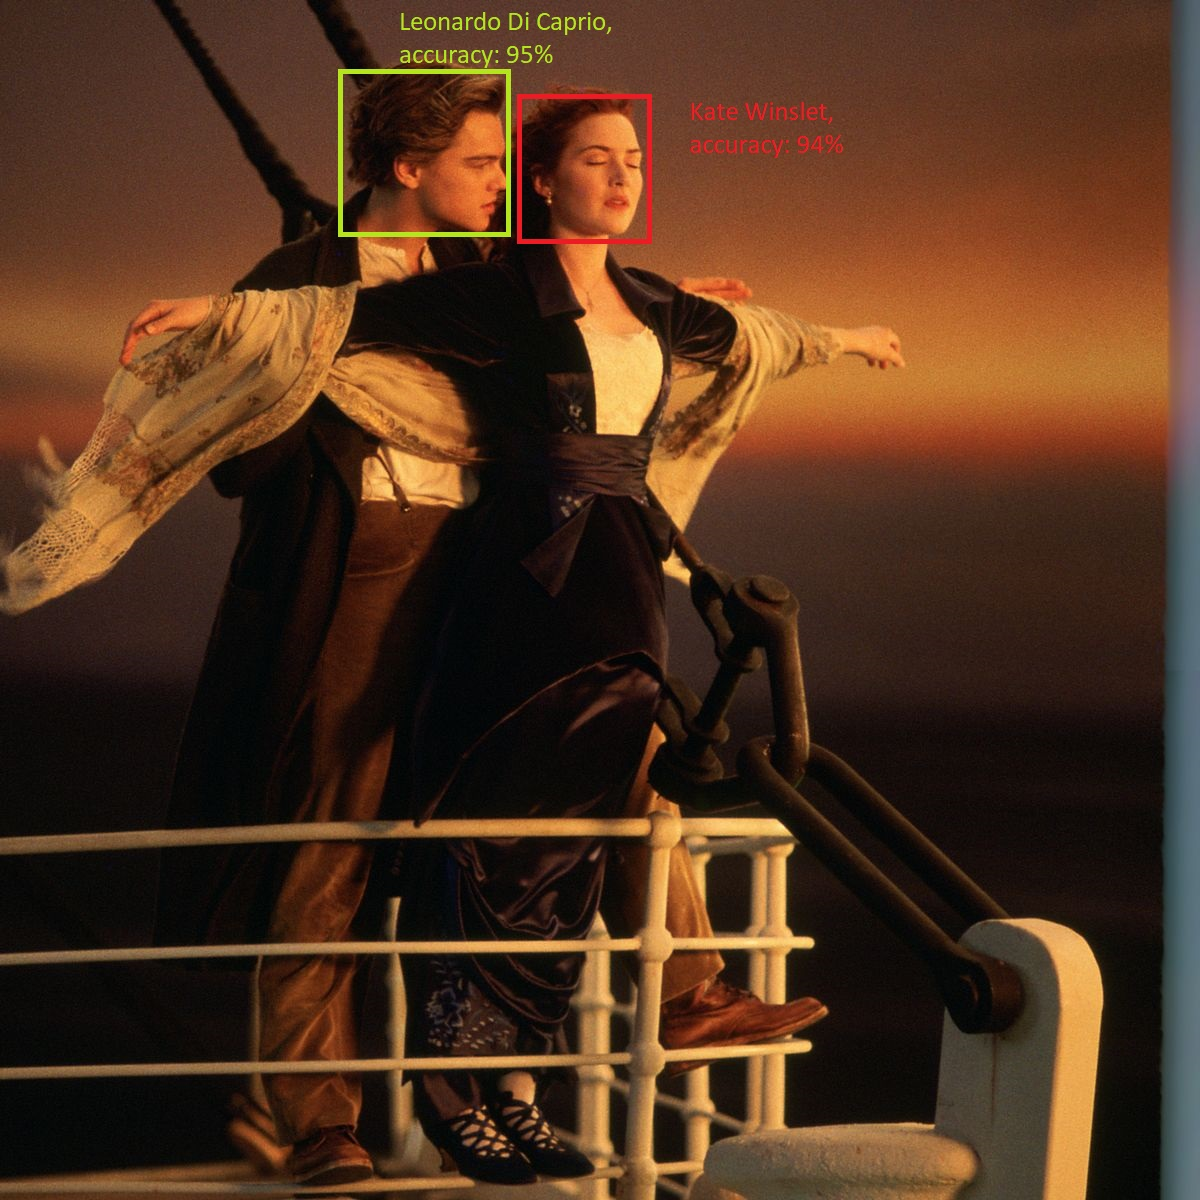
\includegraphics[scale=0.33]{intro1.jpeg}  
\hspace*{.4in}
{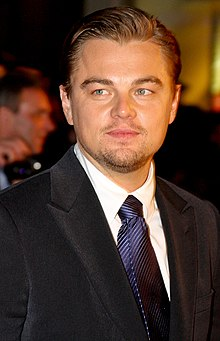
\includegraphics[scale=0.32]{intro3.jpeg}} 
\\
\hspace*{.4in} 
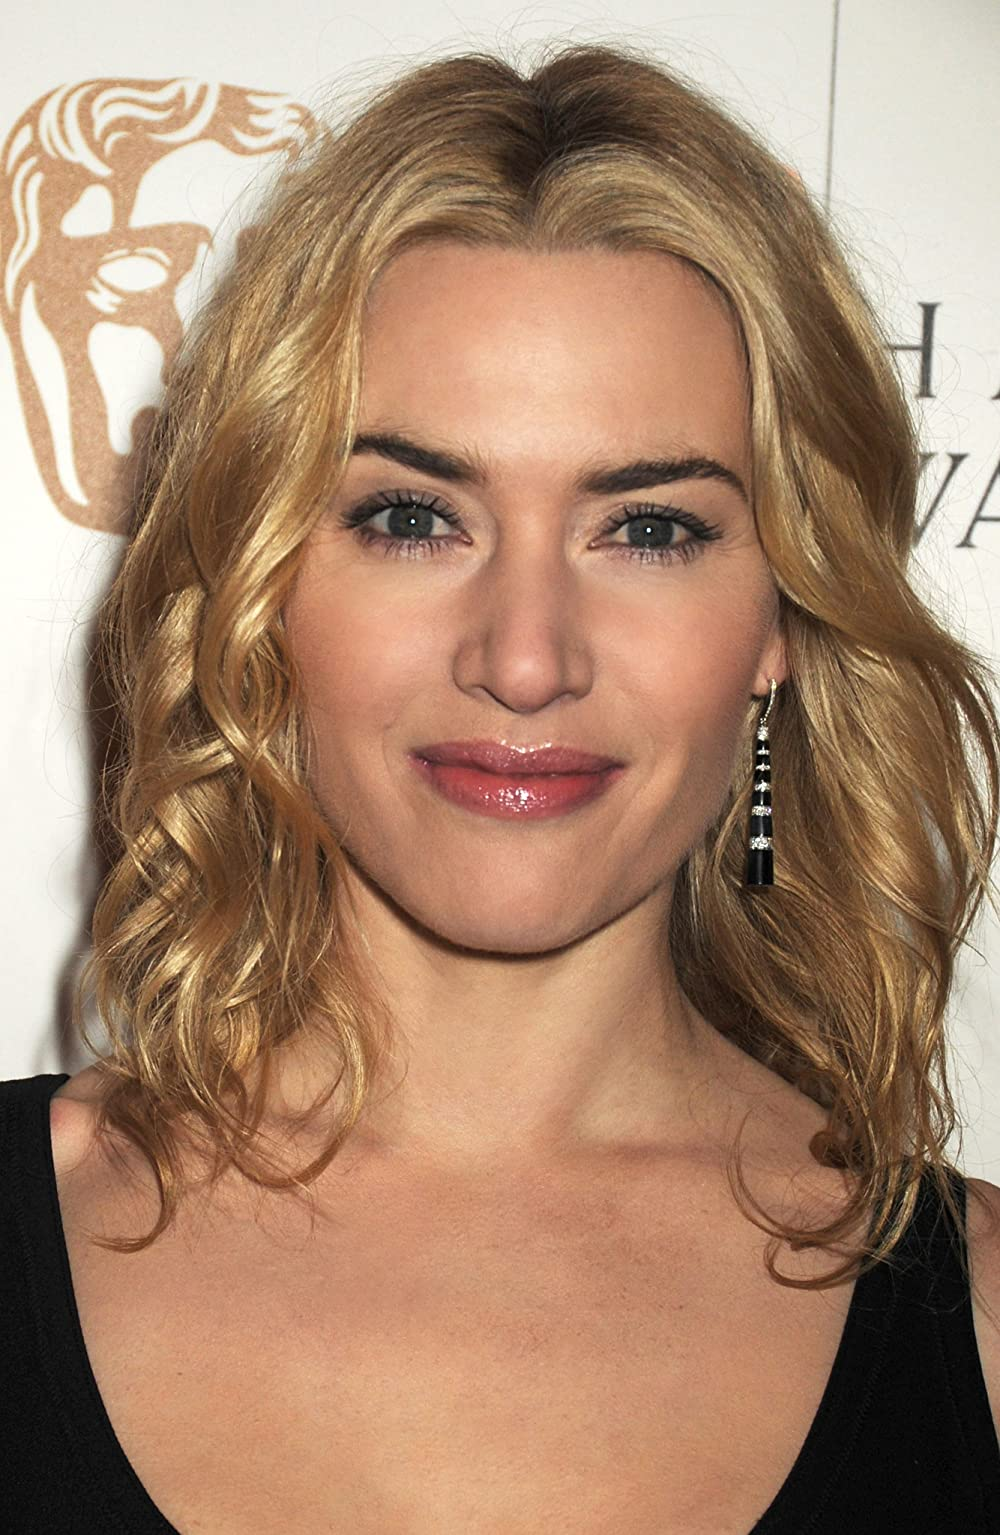
\includegraphics[scale=0.07]{intro2.jpeg}  
\end{multicols}
\end{center}
\vspace*{0.2in}

\section{Steps towards the goal}

\begin{itemize}
  \item Create our own dataset of actor faces, labelled with their name
  \item Process the images with filters and resize them all to the same dimensions
  \item Starting from VggFace weights, fine tune the network on the last two fully-connetected layers
  \item Apply dropout and some heuristics to reach an accuracy higher than 90\% during training on our dataset
  \item Starting from a video, for each possible frame use yoloface to detect the face of the actor
  \item Given a frame and the bounding box of the face, classify the correct names for the actor in the scene.
  \item Retrieval: provide additional photos and information about the actors founded.
\end{itemize}

\end{document}
